\section{How Specific Is the Question Effect?}
\label{sec:crosstask}

To measure how much of the question effect of \S\ref{sec:question} depends on asking for
\emph{this} property, we probe label $A$ while the
prompt asks a different character question $B$ about the same word, at zero shots, so that the self
and cross prompts differ only in the question sentence. Primary cells pair a letter-valued label
with a digit-valued question or the reverse, so $B$'s answer can never equal $A$'s label; cells
whose question arm is not at least 0.05 above the neutral arm are excluded. The two term-label tasks
(\texttt{extraction}, \texttt{letter\_before}) need their query term in every prompt, which we carry
as a bare note line (\texttt{Note the 3rd position.}); they form a secondary arm because the prompt
then differs in two elements.

We split the total question effect (self $-$ neutral) into three additive parts: the generic frame of
awaiting an answer (continuation $-$ neutral), a wrong-property character question
(cross $-$ continuation), and the specific question (self $-$ cross). Figure~\ref{fig:crosstask}
shows the shares.

\begin{figure}[tb]
  \centering
  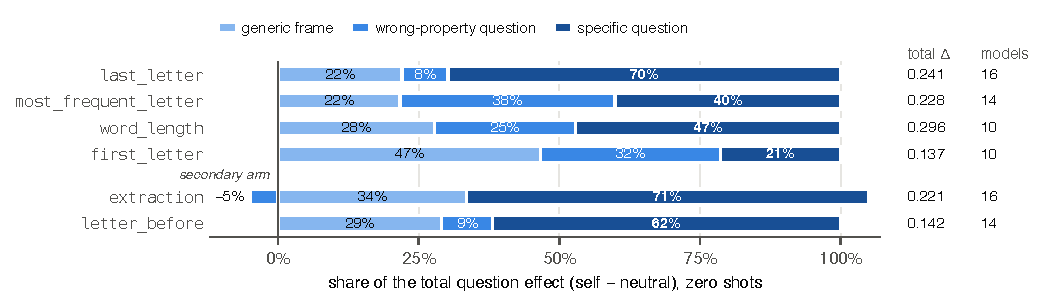
\includegraphics[width=\linewidth]{fig_crosstask.pdf}
  \caption{Decomposition of the question effect at zero shots, zero-leak cells, held-out layer
    selection: shares of the total $\Delta$ (self $-$ neutral, above-majority scale; right), with a
    negative share drawn left of zero. All 16 models were run; ``models'' counts those with at least one qualifying cell. Below the gap: the
    secondary term-label arm. The continuation floor is joined per (model, set, task) from the
    word-position runs, whose example draws differ from the cross-task runs'. Values and cell counts
    in Table~\ref{tab:crosstask}.}
  \label{fig:crosstask}
\end{figure}

For \texttt{last\_letter} and \texttt{extraction}, about 70\% of the effect requires asking for the
property itself; a wrong character question adds almost nothing ($8\%$ and $-5\%$).
\texttt{letter\_before} is similar (62\% specific, 9\% wrong-property). For
\texttt{most\_frequent\_letter}, a wrong character question already delivers 38\% and the specific
question 40\%, so a substantial part of its effect is shared by character questions in general.
\texttt{first\_letter}, whose answer position is near ceiling without any question
(\S\ref{sec:question}), is dominated by the generic frame. Preliminary runs with a peak-over-layers, warm-started estimator gave 70\%, 40\% and 72\% for
\texttt{last\_letter}, \texttt{most\_frequent\_letter} and \texttt{extraction}, within two percentage
points of the present values.

Every cross prompt is itself a character question about the same word, so this design measures how
specific the question effect is to the property asked. It does not separate a general character
routine from property-specific routing, and we draw no conclusion about mechanism from it.
